\documentclass[12pt]{article}

\usepackage{amsfonts}
\usepackage[english]{babel}
\usepackage[a4paper, total={14cm, 26cm}]{geometry}
\usepackage{graphicx}
\usepackage{listings}
\usepackage{multicol}
\usepackage{tabularx}
\usepackage{xcolor}

\definecolor{codegreen}{rgb}{0,0.6,0}
\definecolor{codegray}{rgb}{0.5,0.5,0.5}
\definecolor{codepurple}{rgb}{0.58,0,0.82}
\definecolor{backcolour}{rgb}{0.95,0.95,0.92}

\lstdefinestyle{mystyle}{
    backgroundcolor=\color{backcolour},
    commentstyle=\color{codegreen},
    keywordstyle=\color{magenta},
    numberstyle=\tiny\color{codegray},
    stringstyle=\color{codepurple},
    basicstyle=\ttfamily\footnotesize,
    breakatwhitespace=false,
    breaklines=true,
    captionpos=b,
    keepspaces=true,
    numbers=left,
    numbersep=5pt,
    showspaces=false,
    showstringspaces=false,
    showtabs=false,
    tabsize=2
}

\lstset{style=mystyle}

% Prefix
\title{TerraSearch: An Information Retrieval System Approach for multi-modal Documents}
\author{Jannik Schmied}
\date{\today}

% Start: Document
\begin{document}

\maketitle

% Abstract
\textbf{\abstractname}

Multi-modal documents, in this case defined by the use of different types of writing tools (handwriting, typewriter, etc.), pose a particular challenge for optical character recognition (OCR) software. In the context of this work, a human-in-the-loop approach was conceptually described and implemented. Research has shown, that a semi-automatic procedure, where good-quality documents are batch-processed whereas documents not meeting quality requirements are manually processed by a human supervisor, works best.


\section{Motivation}
\label{sec:motivation}

Over the last couple of decades, significant progress has been made in the field of digitalization. However, many documents still remain to be digitized. It would be even more beneficial if these documents were not merely scanned and archived on a hard drive, but rather indexed and made searchable using a search engine like Google or Bing. The data for this project was provided by the German mining industry, and the documents contained various information such as ground samples, associated calculations, soil composition, and technical metadata, such as \textit{Gauß-Krüger-Coordinates}. These documents were created using a typewriter and supplemented with handwritten notes.

\section{Concept}
\label{sec:concept}

Initially, a volume of approximately one thousand documents containing an average of three pages each was supplied. Upon examining the scans, several challenges became apparent. Firstly, the fact that typewriting and handwriting are combined on a single page indicates that the default OCR model is likely reaching its limits, making a dedicated training necessary. Additionally, the documents were written using different typewriters on the one hand and supplemented with many distinct handwritings on the other. Another challenging circumstance is the significant variation in the quality of the scans. While some are excellent, others are bleached, skewed, have visible signs of aging or all of the above, resulting in direct \textit{optical character recognition} (OCR) being insufficient in many cases. As a result, all documents must be preprocessed to achieve the best possible starting point for further processing.

Subsequently, the content of the document itself should be parsed to extract relevant information. First and foremost, metadata such as the date and location of the document must be identified with the aim of using them later for visualizations. The collected data will then be stored within a database, where further indexing will also take place. In this process, the use of a spell-checking framework should be tested to potentially improve the outcome of the OCR process.

All interaction will take place through a web-based user interface, ensuring maximum compatibility without the need to write dedicated software for every major operating system. The initial deployment will be executed using the Docker container infrastructure, making updates very easy to deploy.

The research on which the documents are based was carried out mostly in Eastern Germany during the 1960s. Since then, changes have been made to city and street names. Therefore, a framework must be found to transform those old addresses into their modern terms.

Keeping in mind all the challenges identified so far and respecting the requirements of a well-searchable and usable software, a \textit{human-in-the-loop} approach seems to fit very well in this case.

\section{Technical Implementation}
\label{sec:implementation}

Following the presented concept, a flow chart was created to visualize the solution (see Figure \ref{fig:flow-chart}).

\begin{figure}[ht]
    \centering
    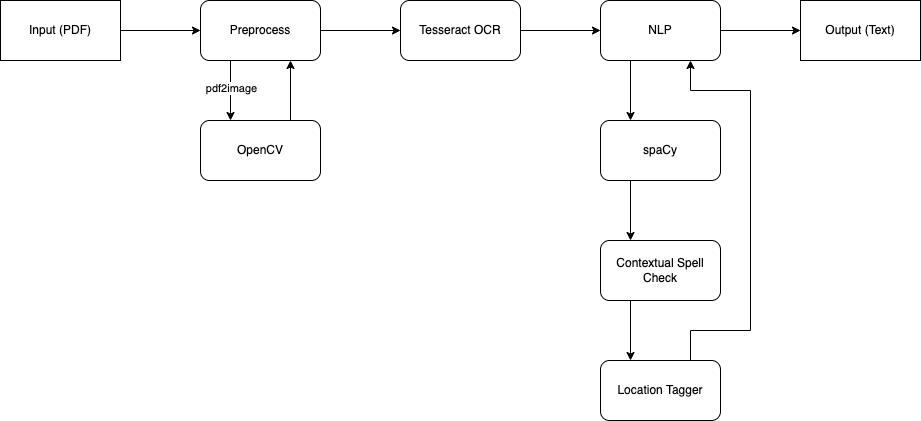
\includegraphics[width=400px]{terrasearch-flow-chart.drawio.png}
    \caption{Flow chart}
    \label{fig:flow-chart}
\end{figure}

\noindent The application consists of four Docker containers, with build instructions defined in the project's docker-compose file. Several necessary environment variables are stored separately in the corresponding .env file.

After starting the build process, the containers are built and started in chronological order, with each depending on its direct predecessor, whose health status is checked beforehand. First, the backend setup is deployed, holding the configuration for all present and future Elasticsearch nodes belonging to the database cluster. Currently, there is only a single node, which is set up afterward. For extended configuration and debugging purposes, a Kibana instance is deployed. The last container holds the Flask web application, including OpenCV and Tesseract.

\subsection{Document Pre-processing}
\label{ssec:preprocessing}

For document preprocessing, every page of the target document will be first converted to an image and then read in as numpy array. From there, OpenCV is used to perform several augmentation operations (see Listing \ref{lst:img-preprocessing}). Hereby, tests have shown, that the \textit{adaptiveThreshold} parameter had the overall highest impact on the OCR outcome. The following arguments are taken by the function:

\begin{lstlisting}[language=Python, label=lst:adaptiveThreshold, caption={OpenCV adaptiveThreshold Function}]
cv2.adaptiveThreshold(img, 
                      max_value, 
                      adaptive_method, 
                      threshold_method, 
                      block_size, 
                      C)
\end{lstlisting}

\noindent Apart from the block\_size parameter, another parameter, C, needs to be provided. After calculating the gaussian-weighted sum of the neighbors, which is done when specifying THRESH\_GAUSSIAN\_C as adaptive method, C is finally deducted.

Since it appears to depend mainly on these two parameters, an empirical test was conducted on five documents with varying quality. The resulting text was then compared to a manual transcript to determine the corresponding match ratio, which is visualized in  Figure \ref{fig:test-bsc}. Across all documents, the overall best ratio (0.3624) was achieved with $ blocksize = 53 $ and $ C = 18 $.

\begin{lstlisting}[language=Python, label=lst:img-preprocessing, caption={OpenCV image processing}, float, floatplacement=H]
def preprocess(image, blocksize: int = 53, constant: int = 18):
    image = cv2.resize(image, None, fx=2, fy=2, interpolation=cv2.INTER_LINEAR)
    img_gray = cv2.cvtColor(image, cv2.COLOR_BGR2GRAY)
    image = img_gray
    image = cv2.dilate(image, np.ones((7, 7), np.uint8))
    img_bg = cv2.medianBlur(image, 21)
    image = 255 - cv2.absdiff(img_gray, img_bg)
    image = cv2.normalize(image, None, alpha=0, beta=255, norm_type=cv2.NORM_MINMAX, dtype=cv2.CV_8UC1)
    image = cv2.adaptiveThreshold(image, 255, cv2.ADAPTIVE_THRESH_GAUSSIAN_C, cv2.THRESH_BINARY, blocksize, constant)
    return image
\end{lstlisting}

\begin{figure}[ht]
    \centering
    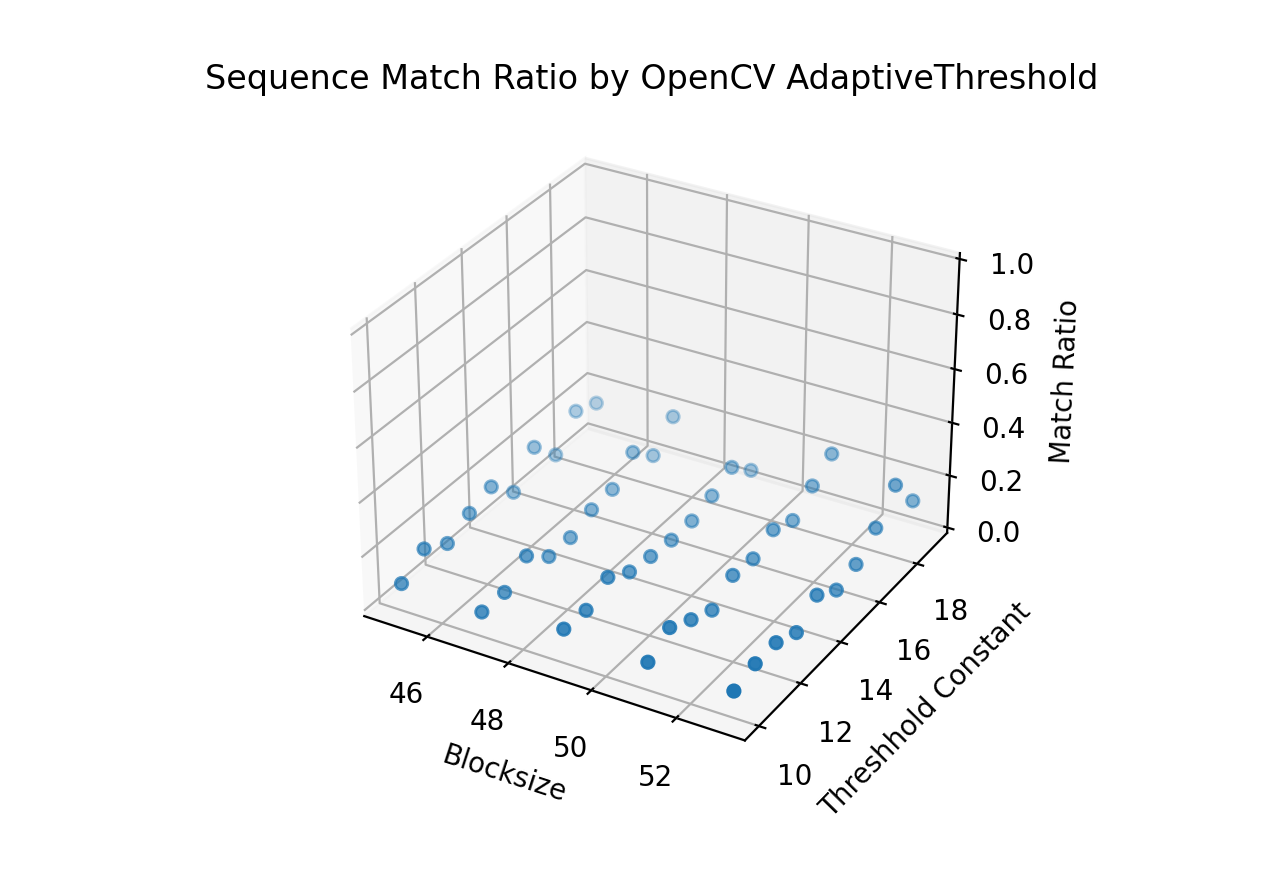
\includegraphics[width=250px]{opencv-adaptive-th.png}
    \caption{Accuracy by Adaptive Threshold Parameter (relevant excerpt)}
    \label{fig:test-bsc}
\end{figure}

\subsection{OCR}
\label{ssec:ocr}

\textit{Tesseract}, Google's OCR engine, is utilized for optical character recognition of the digitized documents. Tesseract comes with a pre-trained model for the German language, which is trained on numerous fonts. However, the accuracy of OCR varies depending on the quality of the document, and different types of documents pose different challenges. Initially, a mean accuracy of 0.3624 was achieved. To enhance accuracy, Tesseract was retrained with eight documents containing a total of 24 pages. The development of accuracy during the training process is depicted in Figure \ref{fig:ocr-accuracy}. While typewritten texts are mostly recognized accurately, handwritten notes still present a challenge due to the lack of sufficient training data for every type of handwriting. Therefore, such passages have to be manually corrected by a human supervisor.

To control Tesseract from Python, the pytesseract library is used. The PDF that is passed is handled page by page. First, the current page is converted into an image file. This is then written into a numpy array and prepared using OpenCV. Finally, the actual OCR is carried out using the image\_to\_string function.

\begin{figure}
    \centering
    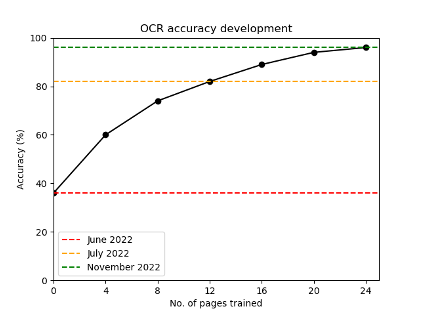
\includegraphics[width=200px]{ocr-accuracy.png}
    \caption{OCR accuracy development over time}
    \label{fig:ocr-accuracy}
\end{figure}

\subsection{NLP}
\label{ssec:nlp}

The main goal of Natural Language Processing (NLP) is to enable computers to process and comprehend natural language, thereby gaining insights from text data and automating tasks that require language understanding. To achieve this, the Python \textit{spaCy} library is utilized. During the execution of the program, the text obtained from OCR goes through several stages within the NLP pipeline. After the initial tokenization, spaCy's \textit{contextualSpellCheck} add-on is utilized to correct minor spelling errors. Following this, the locationtagger library is used to extract specified locations, extending the core functionality of spaCy. To handle the fundamental changes to the German zip code system accompanying the reunification in 1990, a mapping stored in a CSV file is used to transform all zip codes into their modern equivalents. In most cases, this enables the Google Maps Geocoding API to identify the location and return its coordinates.

\subsection{Data storing and indexing}
\label{ssec:database}

To store the data, a single-node \textit{Elasticserach} cluster is used. Inside the database, there is a dedicated index set up for the application. Every entry of the index contains, next to the actual document data, a set of metadata, mainly location. The complete index schema is disclosed in Listing \ref{lst:es-ocr-index}. If scaling becomes necessary in the course of further development, this can be done easily by adding another Elasticsearch container to the docker-compose file.

\begin{lstlisting}[language=Python, label=lst:es-ocr-index, caption={Elasticsearch ocr index}, float, floatplacement=H]
"properties": {
    "document_pdf": {
        "type": "nested",
        "properties": {
            "file_name": {"type": "text"},
            "raw_file": {"type": "text"},
            "pages": {"type": "integer"},
            "signature": {"type": "text"}
        }
    },
    "document_ocr": {
        "type": "nested",
        "properties": {
            "page_number": {"type": "integer"},
            "page_content": {"type": "text"}
        }
    },
    "document_metadata": {
        "type": "nested",
        "properties": {
            "location": {"type": "geo_point"},
            "timestamp": {"type": "date"}
        }
    }
},
"settings": {
    "number_of_shards": 1,
    "index": {
        "similarity": {
            "default": {
                "type": "BM25",
                "b": 0.75,
                "k1": 1.2
            }
        }
    }
}
\end{lstlisting}

\subsection{User Interface}
\label{ssec:ui}

The Software frontend is built on top of a Python \textit{Flask} web server using basic HTML, CSS and JavaScript and subdivided in multiple sub-pages. 

\subsubsection{Search}
\label{sssec:search}

Upon navigating to the application's address, users are directed to the start page, which features a search bar. Users can submit a query and search the related index using the Best Match approach (BM25). All matching results are returned and displayed. Within the results page, users have the option to view or edit each result individually or access a map view that displays the result set.

\subsubsection{Classify and Sync}
\label{sssec:classify-sync}

To add new documents to the index, there are two options. The first option is to bulk insert all documents located inside the sync directory, as specified in the .env file, which is also displayed on the page. This option is recommended for unimodal text documents with good quality. When initiated, all documents are automatically processed and sent to the database without requiring user interaction. For more complex documents, the single classification option should be used. Unlike bulk insertion, the processed document is displayed to a human supervisor, who can correct the result if necessary and then approve it. On the results page, which is equivalent to the edit page discussed in Section \ref{sssec:search}, supervisors can also add metadata and include or remove locations.

\subsubsection{Map}
\label{sssec:map}

For a better understanding of the location distribution, the map by default displays all transformed locations from the index. When users hover over or left-click a pinpoint on the map, an excerpt of the document and a direct link are shown. Currently, the application uses Google Maps API. Initially, OpenStreetMaps was considered, but Google's API proved to be more efficient in converting addresses and offered reverse location search with its Geocoding API. This feature enables natural language locations to be mapped to geographical coordinates.

\section{Conclusion}
\label{sec:conclusion}

Overall, the goal of building a system to semi-automatically digitize documents and index them to make them searchable has been achieved. However, there are several areas that require further attention. Google's APIs are managed via their Google Cloud Platform. As a result, the use of the services creates an additional dependency, which limits the intended universality. To address this issue, a more suitable mapping framework, such as \textit{Plotly} or \textit{GeoEngine}, should be adopted to extend visualization possibilities beyond what is currently available. 

Another area that requires attention is location transformation. Although Google's Geocoding does a decent job of transforming locations by simply changing the zip code, there is still approximately a ten percent mismatch in the results. Further improvements are needed for the location extraction itself as the majority of documents list not only the location of the actual examination but also the address of the executing company. While this is not a problem when supervising the documents manually, these locations are not removed when bulk inserting. Hence, implementing a blacklisting system or something similar is necessary to address this issue.

Additionally, the user interface is currently rudimentary and requires significant improvement. For compliance with common design standards, the use of a dedicated framework should be considered. In order to further increase usability, the user interface should be improved in terms of adaptation to certain device types and accessibility.

% Bibliography
% \newpage

% \bibliography{main}
% \bibliographystyle{ieeetr}

\end{document}
